% Chapter 5
\chapter{跨分辨率遥感影像计数实验及分析}
\section{实验设计}
本设计探究的是跨分辨率遥感影像的计数问题,在跨分辨率车辆计数数据集上,训练本文设计的网络,测试其性能。数据集中共包含了拍摄于同一位置不同时间的192 张极低分辨率图像和 8 张高分辨率图像,低分辨率图像中包含8张和高分辨率图像再同一天拍摄的图像。如何通过少量的高分辨率图像的计数结果,得到可以在低分辨率图像上做出准确计数估计的模型就是本设计的目标。本设计基于CRVC-Net骨架网络,通过独特设计的3个注意力门,更好的综合了从高分辨率及其余两个时间的低分辨率图像的特征信息,逐层与解码器输出进行计算,改进输出效果。

\section{模型训练}
在训练阶段,四张图像输入到网络中。第一输入是\( I^{LR}\),低分辨率图像用于在骨架中生成车辆分割。第二输入是相应的高分辨率图像\( I^{HR}\),起到空间引导的作用。\( I^{LR}\)和\( I^{HR}\)应该在8对相应的低分辨率和高分辨率图像中选取。我们使用其中的7对进行训练,1对进行测试。第三和第四输入是一对低分辨率图像,即\( I^{LR}_{close}\)和\( I^{LR}_{far}\),以强调时间连续性。\( I^{LR}_{close}\)选为与\( I^{LR}\)日期最接近的图像,而\( I^{LR}_{far}\)在图像集中随机选取,与\( I^{LR}\)的时间差超过50天。由于低分辨率和高分辨率图像对数量较少,为了增强鲁棒性,将训练图像裁剪为32×32的补丁后,通过旋转90度、180度和270度,上下左右翻转,将训练集扩大至4000个图像补丁。测试集扩增到1000个图像补丁。在解码器的上采样过程中,使用U-Net结构将上采样的图像与相应比例的特征图跳跃连接。网络输出与原始图像补丁大小相同的32×32的最终分割图。由于训练集是通过旋转和翻转方法生成的,最终的分割结果应该是来自同一图像的各种增强图像的平均值。然后将32×32的补丁拼接成所需的图像大小,以获取整个停车场区域的图像。在测试阶段,只需将\( I^{LR}\)输入到分割骨架中,输出即为车辆分割图。考虑到起重机的数量太少,对分割结果影响不大,我们排除了这一类别,训练和测试阶段只涵盖轿车、小型货车、大型货车和背景四类。

本方法先得到从低分辨率图像得到的分割图,然后据此估计出覆盖率,再由覆盖率通过回归模型估计出最总计数结果,因此主要从以下三个维度度量模型性能:
\begin{enumerate}    
    \item 测试模型在低分辨率(LR)图像上的分割结果,与相应的高分辨率(HR)图像的真实标注进行比较。
    \item 在所有低分辨率图像上测试的车辆覆盖率结果,与人工标注进行比较。
    \item 测试模型在低分辨率图像上的计数结果,与相应高分辨率图像的真实标注进行比较。
\end{enumerate}

\section{分割精度测试}
以同一日期的高分辨率图像的分割图作为标注,本设计在各种网络模块的组合上测试了分割精度。采用像素精度(Pixel Accuracy,PA)来定量评估分割精度。它表示所有像素中正确分类的比例。
\begin{equation}
    P A=\frac{\sum_{i}^{k} p_{i i}}{\sum_{i}^{k} \sum_{j}^{k} p_{i j}}
\end{equation}

假设有\(k+1\)个类别(包括\(k\)个目标类别和1个背景类别),\(p_{ij}\)表示属于类别i但被预测为类别j的像素数量。因此\(p_{ii}\)代表类别为i预测结果也为i的真阳性(TP),\(p_{ij}\)代表类别为i预测结果也为i的假阳性(FP),\(p_{ji}\)代表类别为i预测结果也为i的假阴性(FN)。
基于真阳性(TP)、假阳性(FP)和假阴性(FN),为了更全面的度量该方法在分割方面的性能,通过使用了如召回率(Recall)、精确度(Precision)和F1分数等指标来进一步指示估计精度。\begin{equation}
    \text { Recall }=T P /(T P+F N)
\end{equation}
\begin{equation}
    \text { Precision }=T P /(T P+F P) 
\end{equation}
\begin{equation}
    F 1=2 T P /(2 T P+F P+F N)
\end{equation}结果列在表~\ref{tab:evaluation}中。本文的方法在召回率、精确度和F1分数上均有一定提高。
\begin{table}[h]
    \centering
    \caption{召回率、精确度和F1分数}
    \label{tab:evaluation}
    \begin{tabularx}{\textwidth}{CCCCCCC}
      \toprule
      模型 & 真阳性 & 假阴性 & 假阳性  & 召回率 & 精确度 & F1分数   \\
      \midrule
      CRVC-Net   & 2027  & 2194 & 1037 & 48.0\% & 66.2\% & 0.556 \\   
      本文模型   & 2134  & 2149 & 975 & 49.8\% & 68.6\% & 0.577 \\   
      \bottomrule
    \end{tabularx}
\end{table}


\subsection{消融实验}
为了验证并解释模块设计的合理性和因果性,针对3种注意力门设计了消融实验。
\begin{enumerate}    
    \item 仅使用CRVC-Net骨架进行训练。
    \item 仅使用自注意力门的CRVC-Net进行训练。
    \item 仅使用跨分辨率注意力门的CRVC-Net进行训练。
    \item 仅使用时间序列注意力门的CRVC-Net进行训练。
    \item 使用自注意力门和跨分辨率注意力门的CRVC-Net进行训练。
    \item 使用自注意力门和时间序列注意力门的CRVC-Net进行训练。
    \item 使用自注意力门、时间序列注意力门和跨分辨率注意力门的CRVC-Net进行训练。
\end{enumerate}
实验的结果如下表所示:
\begin{table}[h]
    \centering
    \caption{注意力门消融实验}
    \label{tab:attentiongate}
    \begin{tabularx}{\textwidth}{CCCCC}
      \toprule
      模型 & 自注意力门SAG & 跨分辨率注意力门CAG & 时间序列注意力门TAG & 像素精度  \\
      \midrule
      CRVC-Net   & \times  & \times & \times & 87.5\% \\
      base+SAG   &\surd   & \times & \times & 87.7\% \\     
      base+CAG   & \times  & \surd & \times & 86.3\% \\     
      base+TAG   & \times  & \times & \surd & 84.8\% \\     
      base+SAG+CAG   & \surd  & \surd & \times & 88.2\% \\     
      base+SAG+TAG   & \surd  & \times & \surd & 87.4\% \\     
      base+SAG+CAG+TAG   & \surd & \surd & \surd & \textbf{88.4\%}  \\     
      \bottomrule
    \end{tabularx}
\end{table}

\subsection{实验结果分析}
从上表~\ref{tab:attentiongate}我们可以发现,单独增加自注意力门可以提升像素估计精度,但单独增加跨分辨率注意力门和时间序列注意力门却对估计精度有负面影响。这可能是因为单独引入高分辨率分支特征虽然在训练集上有助于提升最终估计效果,但对于低分辨率的图像的泛化性能却有所下降。单独引入时间序列注意力门虽然丰富了解码器的输入,但没有高分辨率参照下的其余低分辨率特征,并不能很好的指导模型做出正确的估计,反而影响了模型的性能。同时引入自注意力门和跨分辨率注意力门比较明显的提升了模型的性能,同时引入自注意力门和时间序列注意力门也较先前模型有了明显的提升。同时使用三种注意力门单元的模型取得了最好的像素精度估计,也证明了时间序列注意力门单元设计的有效性。虽然单独添加TAG门的效果不佳,但其作为完整模型的一部分有效的弥补了对于不同时间的低分辨率图像的识别能力的不足。
\section{覆盖率估计测试}
在上一步骤中,通过网络模型可以得到低分辨率图像的分割图像估计,据此可以得出车辆的覆盖率。但是由于只有少量低分辨率图像有对应的高分辨率图像作为标注,大部分低分辨率图像采用人工专家标注的方法来判断模型估计的覆盖率结果。低分辨率图像的覆盖率以5\%的间隔手工标注。考虑到人工标注可能存在一些错误,我们根据两个标注者的标注结果的差对标注进行了一些预处理:差值不超过5\%的标注被认为是准确的,而差值位于10\%左右被认为是可接受的。如果差值大于15\%,则认为发生了来两者标注中可能存在错误,将该值排除并由其他专家进行重新标注。上述规则确保了标签的可信度。然后,使用所有人的平均标签值来评估车辆覆盖估计的准确性。下图~\ref{fig:seg}展示了模型估计覆盖率和人工标注覆盖率。
\begin{figure}[h]
    \centering
    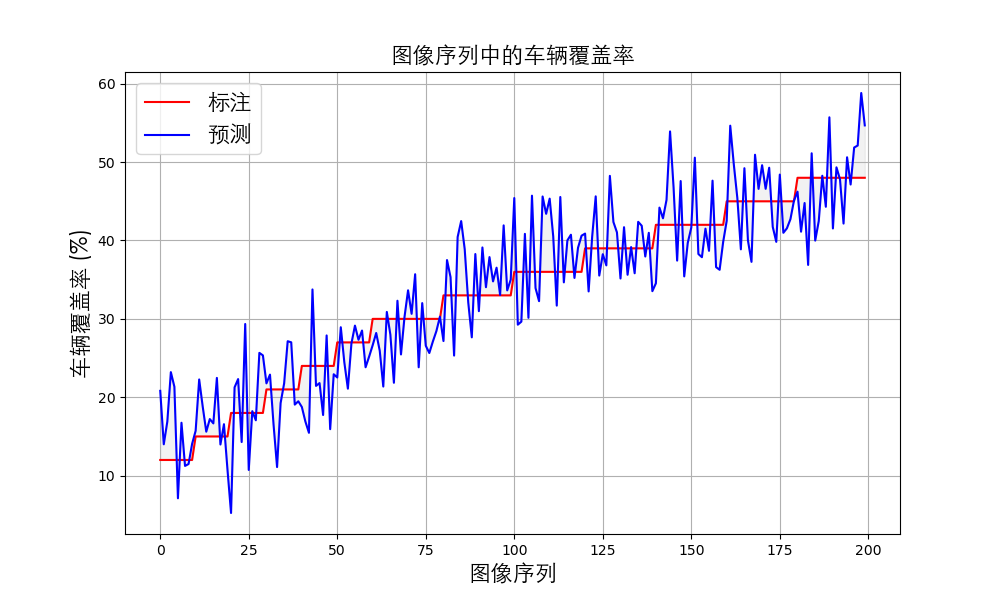
\includegraphics[width=\textwidth]{segmentation.png}
    \caption{覆盖率估计}
    \label{fig:seg}
\end{figure}

\section{车辆计数回归结果测试}
通过车辆覆盖率,可以通过低分辨率图像的大小来计算出车辆区域面积。通过高分辨率图像提供的真值计数信息,可以进行回归分析。本文中对四个车辆类别分别进行了车辆区域面积和车辆数目的回归分析,得到的结果如下图所示。
\begin{figure}[h]
    \centering
    % 第一行两张图
    \begin{subfigure}{0.45\textwidth}
      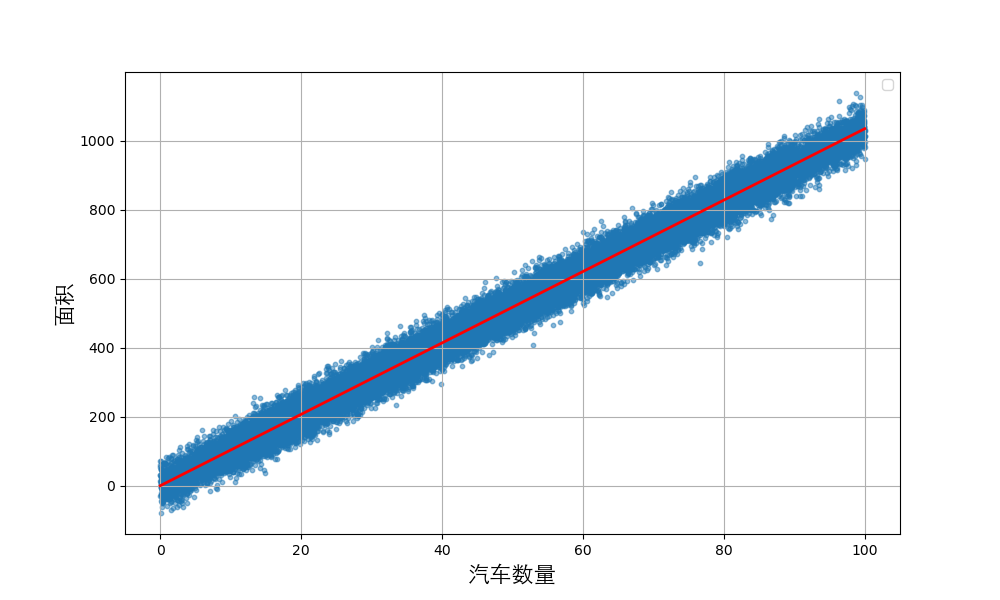
\includegraphics[width=\linewidth]{cars.png}
      \caption{小汽车}
      \label{fig:subfig-a}
    \end{subfigure}\quad % 添加一些间隔
    \begin{subfigure}{0.45\textwidth}
      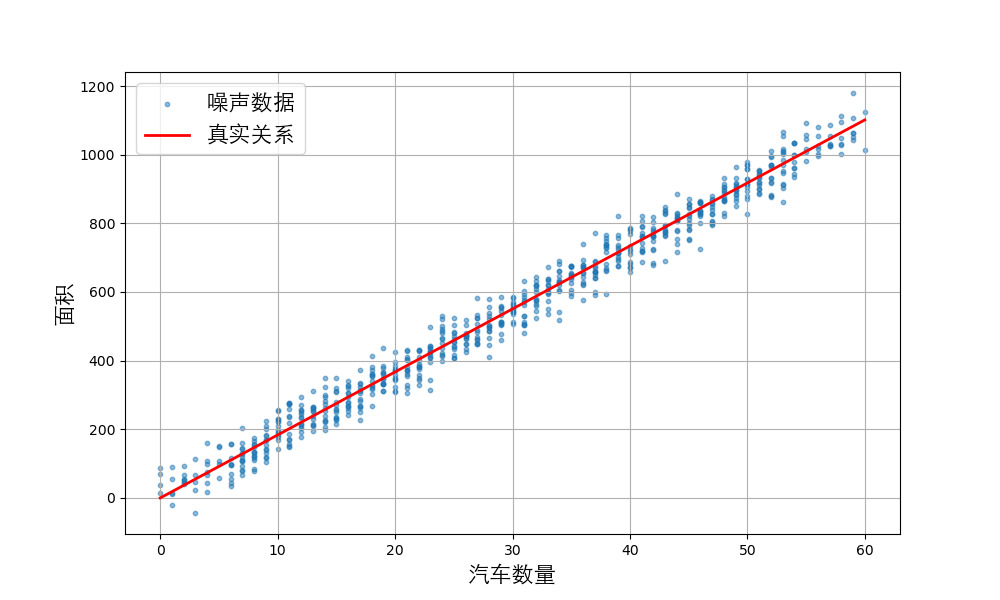
\includegraphics[width=\linewidth]{smalltrucks.png}
      \caption{小型货车}
      \label{fig:subfig-b}
    \end{subfigure}
  
    % 第二行两张图
    \begin{subfigure}{0.45\textwidth}
      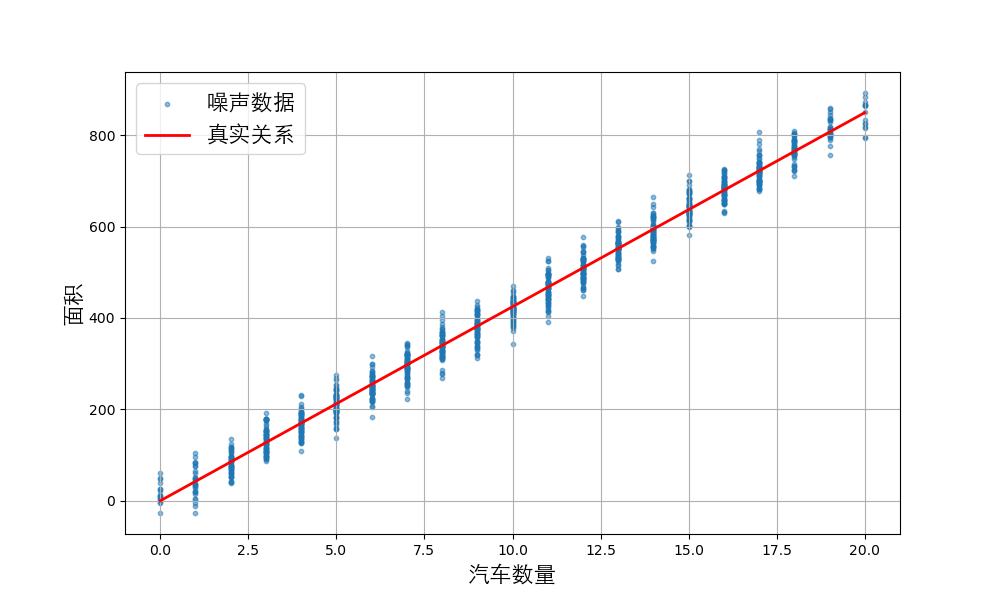
\includegraphics[width=\linewidth]{largetruck.png}
      \caption{大型货车}
      \label{fig:subfig-c}
    \end{subfigure}\quad % 添加一些间隔
    \begin{subfigure}{0.45\textwidth}
      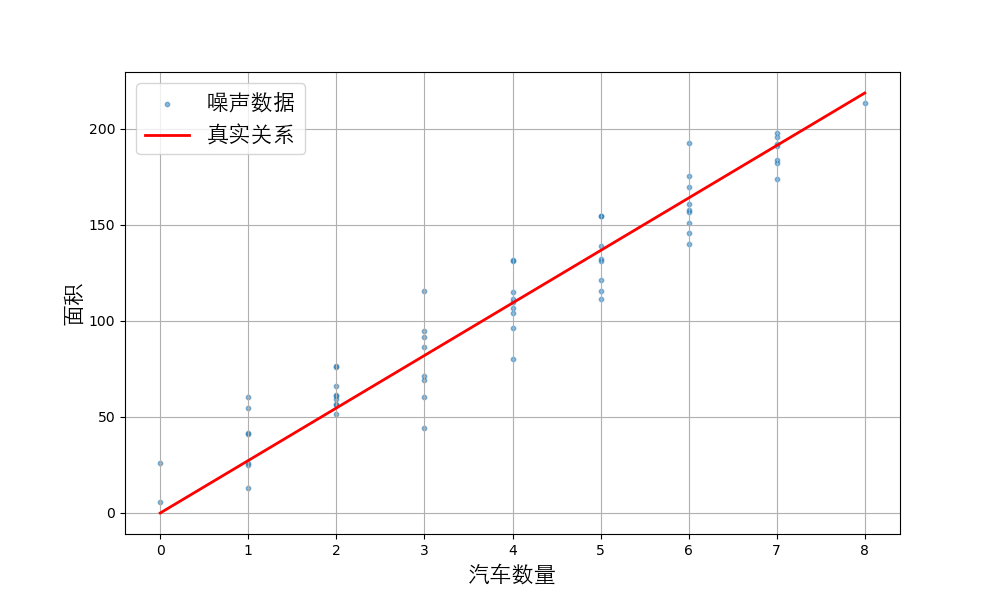
\includegraphics[width=\linewidth]{cranes.png}
      \caption{起重机}
      \label{fig:subfig-d}
    \end{subfigure}
  
    \caption{四种汽车回归计数的结果}
    \label{fig:multi-image}
  \end{figure}

  对于小汽车、小型货车、大型货车和起重机四个类别,回归模型预测的斜率分别为10.353、18.354、42.468和27.323,\(R^2\)分别为0.9867、0.9821、0.9854和0.9376。\(R^2\)大于零且接近一,具有很强的正相关性。

\section{训练细节}
在训练过程中涉及到多个超参数的选择,其中比较重要的是损失函数的权重。模型使用的损失函数如下:
\begin{equation}
    \mathcal{L}=\omega_1\mathcal{L}_{\text {ent }}+\omega_2\mathcal{L}_{\text {dir }}+\omega_3\mathcal{L}_{\text {ser }}
    +\omega_4\mathcal{L}_{\text {FL }}
\end{equation}
为了能够让模型能够先掌握车辆的整体结构及更好的适应数量占据大多数的轿车类别,在前10000个轮次中,将\(\omega_4\)设置为0,将\(\omega_1\)设置为0.5,将\(\omega_2\)设置为0.4,将\(\omega_3\)设置为0.1,以避免对于轿车分类的惩罚。在后续的5000个轮次中,\(\omega_1\)设置为0,\(\omega_2\)和\(\omega_3\),\(\omega_4\)设置为0.5,这时使用焦点损失函数专注于学习大型货车和小型货车类别。这有助于更好的识别小样本类别,同时对于背景类别的也能有更好的区分


\section{局限}
本模型采用的多头注意力门结构确实可以增加模型对数据的理解深度,但同时也会带来一系列局限性和挑战。

首先多头注意力机制通常会导致显著的参数增加。这种参数增加意导致在训练和推理过程中需要更多的内存来存储额外的参数和中间计算结果。这种增加的内存需求可能会限制模型能够处理的最大批量大小。当该方法应用于其他更大规模的数据集上时,参数量及训练时间的影响将更为显著。下表展示了不同模型的参数数量对比,可以直观的观察出参数量的增长。
\begin{table}[h]
    \centering
    \caption{不同模型的参数量}
    \label{tab:parma}
    \begin{tabularx}{\textwidth}{CCCC}
      \toprule
      模型 & 总参数量 & 可训练参数量 & 内存占用  \\
      \midrule
    CRVC-Net& 37,922,787  & 37,916,773 & 144.66MB \\
    CRVC-Net+AG& 50,689,801  & 50,677,897 & 193.37MB \\
    本文模型  & 134,969,540    & 134,956,548 & 514.87MB \\   
      \bottomrule
    \end{tabularx}
\end{table}


参数数量的增加,尽管可以帮助模型学习更复杂的特征,但也可能使模型更容易过拟合,特别是在如CRVC这样的小型数据集上训练时。即使使用图像增广技术,如翻转、缩放和平移,这些操作可能不足以生成模型需要的多样化数据来充分学习并泛化到未见过的数据。
同时大量的参数和复杂的模型结构可能导致优化过程中出现问题,如梯度消失或梯度爆炸,对于参数的调整和优化算法的选择上有着更高的要求。





